% Figure 2 of technical_report.md: the advanced task. Left, our code in the Docker image; right, the
% requests to Apertus through BASE_URL. The numbers are the steps of Section 2.3; a dashed box is a step
% that only some cases take. Steps 1 and 2 run once per booklet, for the first case that needs it.
%
% Build in docs/, with pdflatex and Poppler's pdftocairo:
%
%     pdflatex architecture_advanced.tex
%     pdftocairo -svg architecture_advanced.pdf architecture_advanced.svg
\documentclass[border=6pt]{standalone}
\usepackage[T1]{fontenc}
\usepackage{lmodern}
\usepackage{tgheros}
\renewcommand{\familydefault}{\sfdefault}
\usepackage{tikz}
\usetikzlibrary{arrows.meta,backgrounds,calc,positioning}

\definecolor{ink}{HTML}{1F2937}
\definecolor{muted}{HTML}{4B5563}
\definecolor{lane}{HTML}{F3F4F6}
\definecolor{laneline}{HTML}{D1D5DB}
\definecolor{group}{HTML}{E5E7EB}
\definecolor{apertus}{HTML}{1D4ED8}
\definecolor{apertuslane}{HTML}{EFF6FF}
\definecolor{apertusline}{HTML}{93C5FD}
\pagecolor{white}  % also behind the headings, for a dark page around the SVG

% A box's text: its title, then a line or two of detail
\newcommand{\what}[2]{\textbf{#1}\\[1pt]{\footnotesize\color{muted}#2}}

\tikzset{
  every node/.style={font=\small, text=ink},
  >={Stealth[length=5pt, width=4pt]},
  box/.style={draw=ink!60, fill=white, rounded corners=3pt, align=left,
              inner xsep=11pt, inner ysep=4pt, minimum height=10mm},
  stage/.style={box, text width=70mm},
  call/.style={box, draw=apertus, text width=40mm},
  io/.style={fill=ink!10, rounded corners=7pt, align=center, text width=70mm,
             inner xsep=11pt, inner ysep=3pt},
  number/.style={circle, fill=ink, text=white, font=\footnotesize\bfseries,
                 inner sep=0pt, minimum size=5mm},
  flow/.style={->, draw=ink!60, line width=0.8pt},
  request/.style={->, draw=apertus, line width=0.8pt},
  lanebox/.style={rounded corners=6pt, line width=0.6pt},
  heading/.style={font=\footnotesize\bfseries, anchor=south},
}

\begin{document}
% 1.7 times as large: browsers draw the SVG's points as pixels, which would make its text tiny
\scalebox{1.7}{%
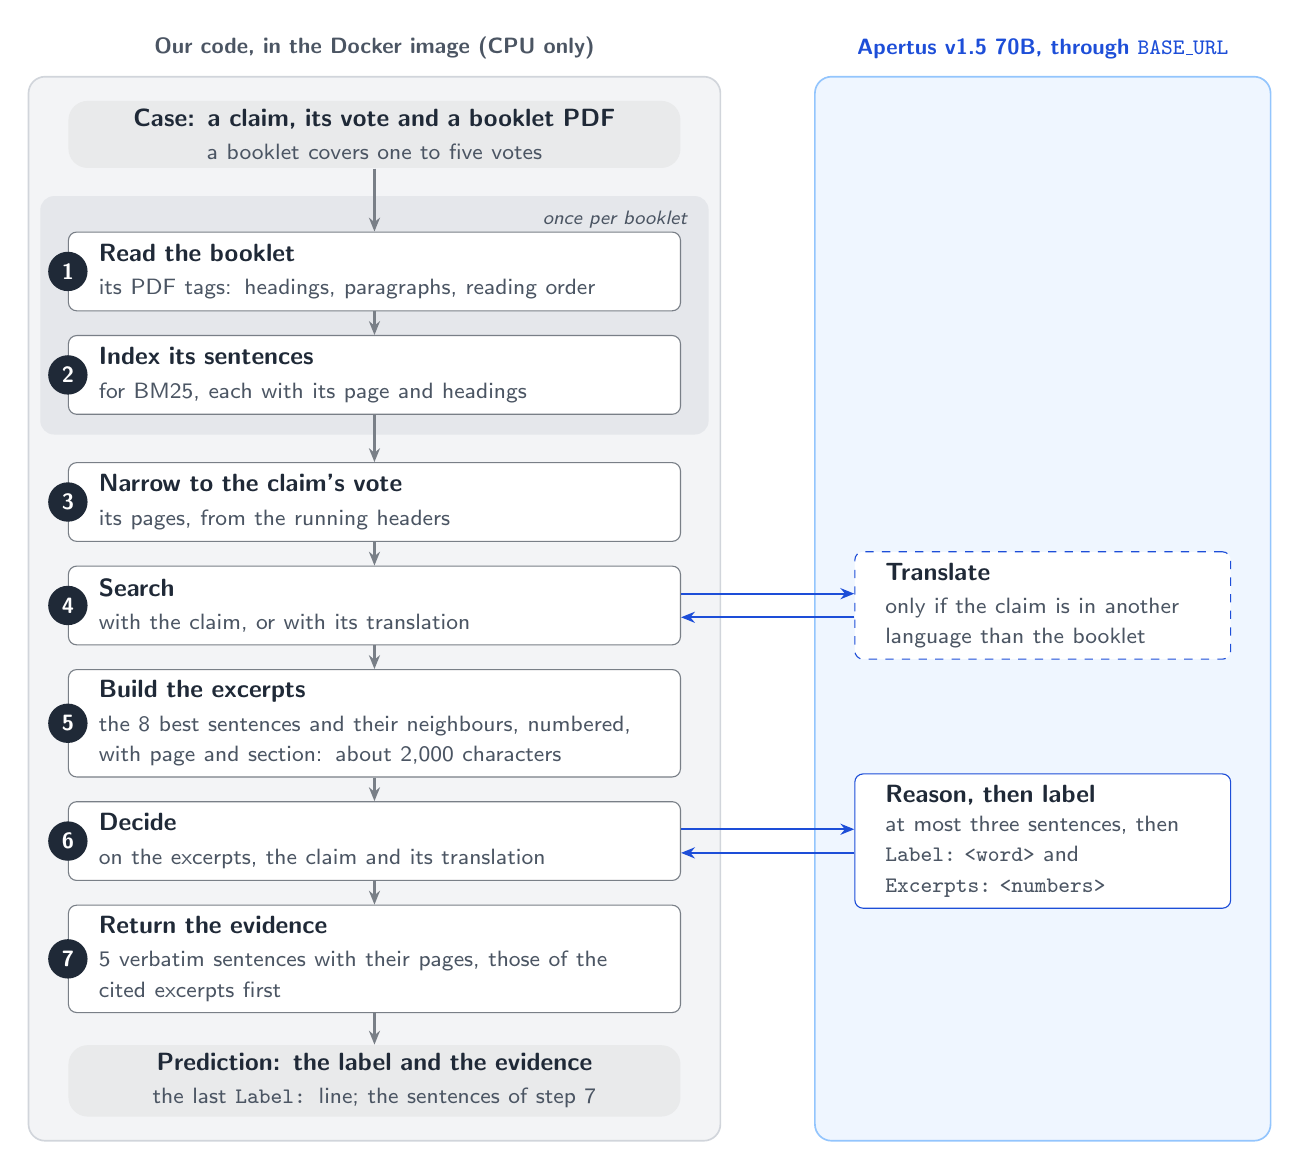
\begin{tikzpicture}[node distance=3mm]
  % Our code, top to bottom
  \node[io] (case) {\what{Case: a claim, its vote and a booklet PDF}{a booklet covers one to five votes}};
  \node[stage, below=8mm of case] (s1)
    {\what{Read the booklet}{its PDF tags: headings, paragraphs, reading order}};
  \node[stage, below=of s1] (s2)
    {\what{Index its sentences}{for BM25, each with its page and headings}};
  \node[stage, below=6mm of s2] (s3)
    {\what{Narrow to the claim's vote}{its pages, from the running headers}};
  \node[stage, below=of s3] (s4)
    {\what{Search}{with the claim, or with its translation}};
  \node[stage, below=of s4] (s5)
    {\what{Build the excerpts}{the 8 best sentences and their neighbours, numbered, with page
     and section: about 2,000 characters}};
  \node[stage, below=of s5] (s6)
    {\what{Decide}{on the excerpts, the claim and its translation}};
  \node[stage, below=of s6] (s7)
    {\what{Return the evidence}{5 verbatim sentences with their pages, those of the cited
     excerpts first}};
  \node[io, below=4mm of s7] (prediction)
    {\what{Prediction: the label and the evidence}{the last \texttt{Label:} line; the sentences
     of step 7}};

  % Apertus, beside the steps that call it
  \node[call, dashed, right=22mm of s4] (c4)
    {\what{Translate}{only if the claim is in another language than the booklet}};
  \node[call, right=22mm of s6] (c6)
    {\what{Reason, then label}{at most three sentences, then\\\texttt{Label:~<word>} and
     \texttt{Excerpts:~<numbers>}}};

  \foreach \n in {1, ..., 7} \node[number] at (s\n.west) {\n};
  \draw[flow] (case) -- (s1);
  \foreach \n [evaluate=\n as \next using int(\n + 1)] in {1, ..., 6} \draw[flow] (s\n) -- (s\next);
  \draw[flow] (s7) -- (prediction);
  \foreach \n in {4, 6} {
    \draw[request] ([yshift=1.5mm]s\n.east) -- ([yshift=1.5mm]c\n.west);
    \draw[request] ([yshift=-1.5mm]c\n.west) -- ([yshift=-1.5mm]s\n.east);
  }

  % Where each runs: the two lanes, as high as the steps; steps 1 and 2 run once per booklet
  \coordinate (top) at ($(case.north) + (0, 3mm)$);
  \coordinate (bottom) at ($(prediction.south) + (0, -3mm)$);
  \begin{scope}[on background layer]
    \path[lanebox, fill=lane, draw=laneline]
      ($(s1.west |- top) + (-5mm, 0)$) rectangle ($(s1.east |- bottom) + (5mm, 0)$);
    \path[lanebox, fill=apertuslane, draw=apertusline]
      ($(c4.west |- top) + (-5mm, 0)$) rectangle ($(c4.east |- bottom) + (5mm, 0)$);
    \path[fill=group, rounded corners=5pt]
      ($(s1.north west) + (-3.5mm, 4.5mm)$) rectangle ($(s2.south east) + (3.5mm, -2.5mm)$);
  \end{scope}
  \node[font=\scriptsize\itshape, text=muted, anchor=north east]
    at ($(s1.north east) + (2mm, 3.9mm)$) {once per booklet};
  \node[heading, text=muted] at ($(s1.north |- top) + (0, 1mm)$)
    {Our code, in the Docker image (CPU only)};
  \node[heading, text=apertus] at ($(c4.north |- top) + (0, 1mm)$)
    {Apertus v1.5 70B, through \texttt{BASE\_URL}};
\end{tikzpicture}}
\end{document}
